\documentclass{article}

\usepackage{amsmath}
\usepackage{natbib}
\usepackage{graphicx}
\usepackage{siunitx}
\usepackage{float}
\usepackage{hyperref}
\newcommand\tab[1][1cm]{\hspace*{#1}}
\date{} 
\begin{document}





\begin{figure}[!tp]
\vspace{-10mm}

\includegraphics[scale=0.8]{ee.png}


\vfil
\hfil \Large \bf MIDDLE EAST TECHNICAL UNIVERSITY
 \hfil
\vfil

\vspace{5mm}
\vfil
\hfil \large \bf  EE464- STATIC POWER CONVERSION-II
 \hfil
\vfil

\vspace{5mm}
\vfil
\hfil \large \bf HARDWARE PROJECT SIMULATION REPORT \hfil
\vfil
\bf

\vspace{23mm}
Mert ZEYBEK    \tab\tab 2167682


Hamza SOLAK \tab\tab2263762


\vspace{5mm}
\small Date: 23/03/2020


\end{figure}

\newpage
\tab\tab
\section*{Introduction}
The aim of this project is to design a dc-dc converter with one of the two topologies. Topologies are flyback converter and forward converter, trade-offs between these topologies is discussed. When we are choosing our topology, we must examine the specification of the project. Every topology have some advantages and disadvantages. We must compare the advantages and disadvantages for choosing right topology. 
\newline \tab After choosing our topology and project specifications, design details of projects are discussed including necessary components, integrated circuits, design of magnetic components with the help of simulation results in this report.

\section*{Topologies}
\subsection*{1)Flyback Converter}
\tab\textbf{a)}

\begin{figure}[H]
\centering
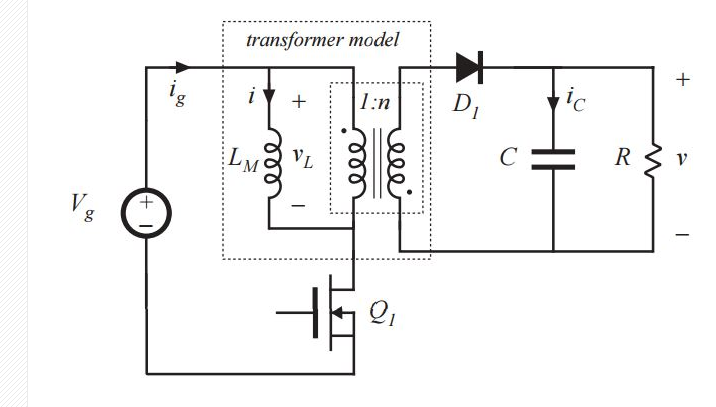
\includegraphics[width=\textwidth]{flyback.PNG}
\caption{Flyback converter circuit schematic.}
\end{figure}
\tab The flyback converter is based on the buck-boost converter.It is isolated buck-boost converter. Isolation provided with transformer.It is simple isolated converter. It's input output relation is shown in the equation below. 
\begin{equation}
    \frac{V_o}{V_d}=\frac{D*N_2}{(1-D)*N_1}
\end{equation}
\subsection*{2) Forward Converter}
\begin{figure}[h]
    \centering
    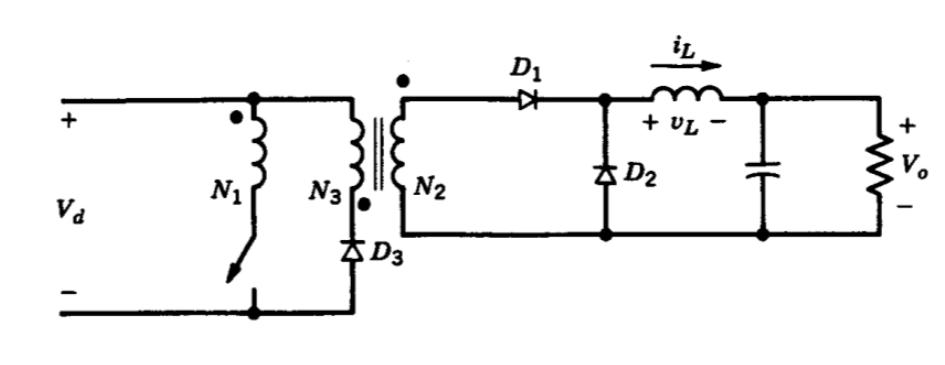
\includegraphics[scale=0.5]{forwardconverter.PNG}
    \caption{Forward converter circuit schematic }
    \label{fig:my_label}
\end{figure}
\tab\textbf{} It derived from buck converter.It uses transformer for increasing and decreasing output voltage. Transformer provides isolation between input and output.Forward converter's input and output relation is shown equation below. 
\begin{equation}
    \frac{V_o}{V_d}=\frac{N_2}{N_1}*D
\end{equation}



 


\subsection*{3) Comparison Between Converter Topologies}

\tab\textbf{a) Flyback Converter} 
\newline
\newline
\tab Flyback converter have advantages over forward converter. It is cheaper than forward converter.It needs small voltage rating mosfet and change in the gain is small. We can design more compact circuit with flyback converter.
\newline
\newline
\tab\textbf{a) Forward Converter} 
\newline
\newline
\tab Forward converter have advantages over flyback converter. It has better utilization of transformer. It provides higher power transformer. In design we can use gapless core. It provides us higher $L_m$ and less ripple. Output inductor and diode ensure continuous output current. It also  can provide higher efficiency. 
\newline
\newline
\tab We choose forward converter because in the specification we need less regulation and better utilization. Forward converter can provide these specifications. Since there is no cost and volume specification, its disadvantages are less important for our project. 

\newpage
\section*{Design Decisions}
\subsection*{1) Magnetic Design}
\tab\textbf{a) Transformer Design}

\tab Our considerations regarding transformer was based on \href{https://www.mouser.com/pdfdocs/2-10.pdf}{Converter Design Note Document by Infineon}. We started with turn ratio decision considering the following formula:
\begin{equation}
    \frac{V_o}{V_i}=\frac{n_3}{n_1}D
\end{equation}
\tab Since we want D value to be smaller than 0.5 so that we do not charge the transformer core at each cycle. If D was larger than 0.5, it would saturate the core which is not desired.
\newline \tab As a result, we decided to have a $\frac{n_3}{n_1}=1.2$ which corresponds to 14.4 V at the output. Considering voltage drops on transistors, diodes and resistive parts of the elements, it will give a voltage less than 14.4 V at practice when minimum input voltage $24 V$ is applied. So, at D close to 0.5, we expect to acquire 10 V output voltage. At maximum input voltage $48 V$, D value becomes $0.17$. It will get smaller once the losses on the system are included. As a result, we get enough range of D to adapt to changes in input voltages. For the sake of simplicity, we chose $n_2$ same as $n_1$, which is usually the case in practical applications.
\newline \tab Next, we considered the following equation in order to avoid saturation of the core:
\begin{equation}
    n_1>\frac{V_{i_{max}}.D_{max}}{B_{sat}.A_e.f_s}
\end{equation}
\tab In order to have a meaningful result from this equation, we need to choose the transformer core so that we can put $B_{sat}$ and $A_e$ values in the equation. We selected to use an E core since their geometrical structure is suitable for three winding application. Considering the E cores that are available in the laboratory, we had two different types of cores, namely Kool Mu and Ferrite. Since we desire to have a high permeability core for Forward Converter, ferrite cores fit better for our application. Between ferrite cores, \href{https://www.mag-inc.com/Media/Magnetics/Datasheets/0P45530EC.pdf}{0P45530EC} is the best solution since it has the largest window area. Although using large core means increase in cost, it ensures us that we are far from saturation and it also enables us to lower frequency, which means better efficiency, which is more important than cost in this project. We also need to select switching frequency. Since our core is large enough, selecting a relatively low frequency will increase efficiency and it will also ease semiconductor device selection. 10 kHZ switching frequency seems optimum for this case. As a result, minimum $n_1$ value can be calculated as follows for core with $B_{sat}=0.3 T $ and $A_e=420 mm^2$:
\begin{equation}
    n_1>\frac{48*0.5}{0.3*420*10^-6*10^4}
\end{equation}

\begin{equation}
    n_1>19
\end{equation}
\tab Since we do not want to increase copper losses, keeping $n_1=20$ is the most suitable choice for our application. It also means that $n_2=20$ and $n_3=24$.
\newline \tab Last thing to consider regarding transformer design is size of the cable. Choosing a cable with too small cross section would not have enough current carrying capability and resistance would be higher which would decrease efficiency. On the other hand, too large cross sectional area would result in too large fill factor.
\newline\tab AWG14, which has $2.08 mm^2$ cross section area and $5.9 A$ current carrying capability is suitable for our application. Fill factor calculation can be seen below:

\begin{equation}
    k_f=\frac{n*A_{cable}}{A_e}=\frac{(24+20+20)*2.08 mm^2}{420 mm^2}=0.317
\end{equation}

\tab Fill factor is small enough proper operation. As a result, AWG14 cable can be used at our transformer.\\

\tab\textbf{b) Output Inductor Design}
\newline \tab At inductor design, we want to limit output current ripple which would also ensure continuous conduction mode. We want to keep the converter in CCM since forward converter's gain changes a lot in DCM. On the other hand, choosing a too large inductor would increase DCR value, which would reduce efficiency. We considered following equations for calculation of our output inductor considering 2 \% ripple rating:
\begin{equation}
    I_{L_O,min}=I_{O,max}*0.02 =4.8*0.02=0.096 A
\end{equation}
Ripple value must be less than twice of this value which is given below:
\begin{equation}
{\displaystyle \Delta }I_{L_o}=(\frac{n_3}{n_1}*V_i-V_o)*\frac{1}{L_o}*t_{on}<0.192 A
\end{equation}
\tab As a result, we need an inductor with $3.8 mH$ inductance in order to meet criteria. This value is relatively high since our switching frequency is small but there are commercial products available at that value as well as we can wind one by ourselves.

\subsection*{2) Closed Loop Control}
\tab Closed loop control is critical in this application since we need supply fixed output voltage to load with changing input voltage. To achieve that, we need to have a feedback from output voltage and adjust duty cycle that drives the transistor accordingly. While doing that, we must not break isolation between input and output. 
\newline \tab In order to achieve that we plan to use an analog integrated circuit, \href{http://www.ti.com/lit/ds/symlink/tl494.pdf}{TL494}. It enables us to control  switching frequency with a single resistor and capacitor. TL494 also has soft start feature, which can be helpful for selecting semiconductor devices with smaller ratings because it helps us to avoid high starting voltages and currents.
\newline \tab One thing to consider while using TL494 is it cannot directly be connected to transistor's gate since it cannot supply enough current to turn on and off the transistor. \href{https://pdf.direnc.net/upload/tlp250-datasheet.pdf}{TLP250} optocoupler connected between TL494 and transistor's gate can solve the issue. For isolation purpose, feedback from the output voltage can also be taken using an optocoupler as well. 
\newline \tab Another issue with TL494 usage is its supply voltage. In order to achieve our task with single power supply, we need to supply the IC from our input voltage. However, constant $15 V$ needs to be supplied to the IC. We need to use a regulator for that purpose if we aim to achieve single supply bonus.

\newpage
\section*{Simulation Results and Component Selections}
\tab We built a Simulink model with our design decisions. For more detailed calculation and component selection, we simulated our topology and devices in Matlab Simulink. Our Matlab circuit schematic is shown in Figure 3. 
\begin{figure}[H]
    \centering
    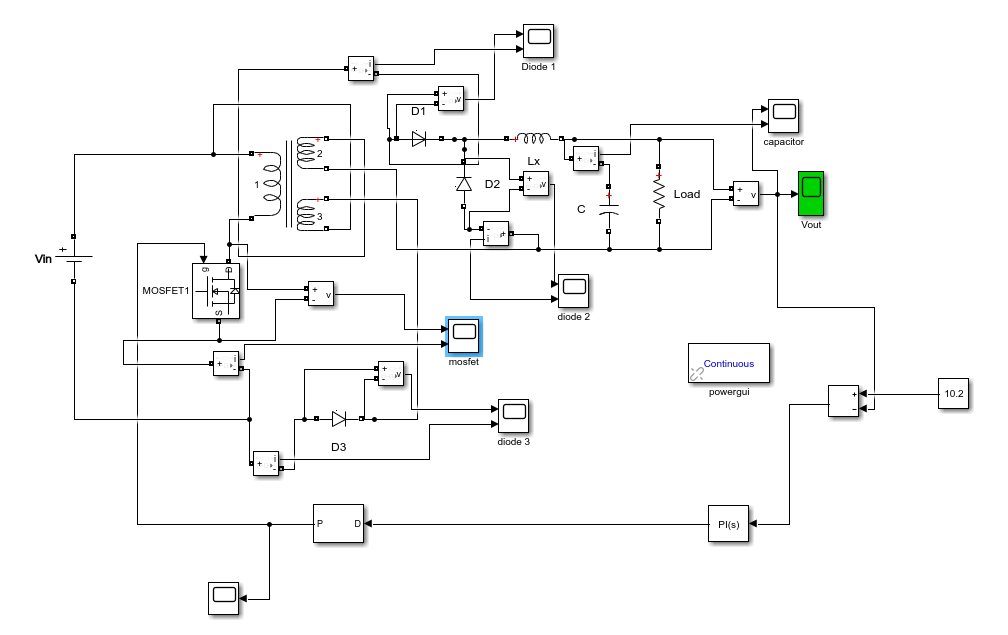
\includegraphics[scale=0.4]{circuit.PNG}
    \caption{Simulink simulation schematic}
    \label{fig:my_label}
\end{figure}
\tab\textbf{a)} Firstly we simulate the case where the input is 48V and output is the 10V. Simulation results are shown below. 
\begin{figure}[H]
    \centering
    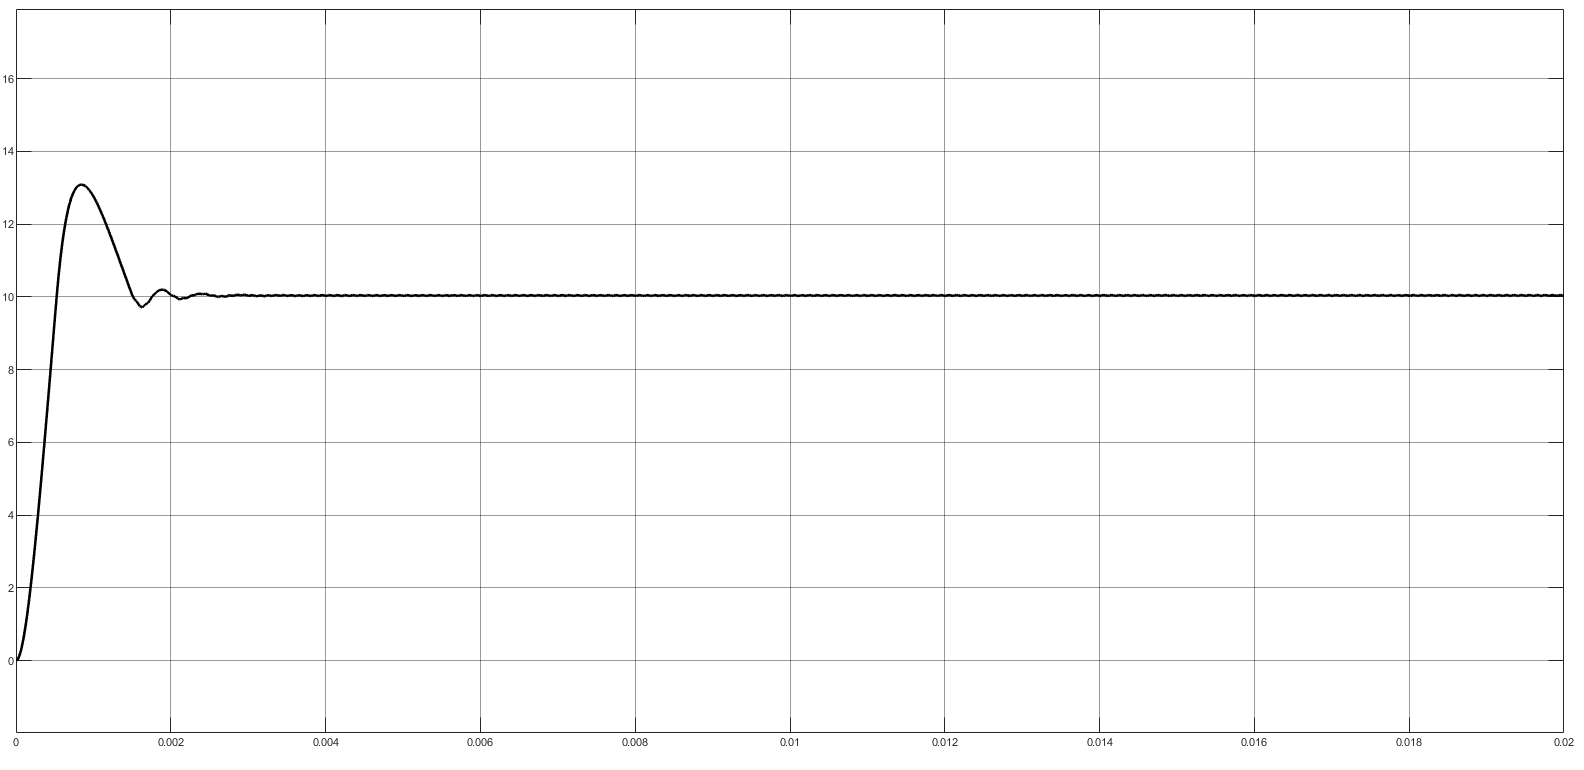
\includegraphics[scale=0.3]{48in.png}
    \caption{Output waveform when input is 48V}
    \label{fig:my_label}
\end{figure}
\newline
\tab Output must be constant at 10V. When input is equal to 48V Our duty cycle must be smallest value due to the specifications.Our smallest duty cycle is $\%$17.584.  $\%$17.584 duty cycle give us 10V when input is 48V.Signal statistics of the output waveform is shown below.
\begin{figure}[H]
    \centering
    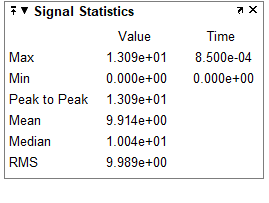
\includegraphics[scale=0.9]{48sinyal.PNG}
    \caption{Output waveform signal statistics when input is 48V}
    \label{fig:my_label}
\end{figure}

\tab In design and component selection currents are important. For choosing current rating of devices we observe currents of devices. Current and voltage waveform of the mosfet shown below. 

\begin{figure}[H]
    \centering
    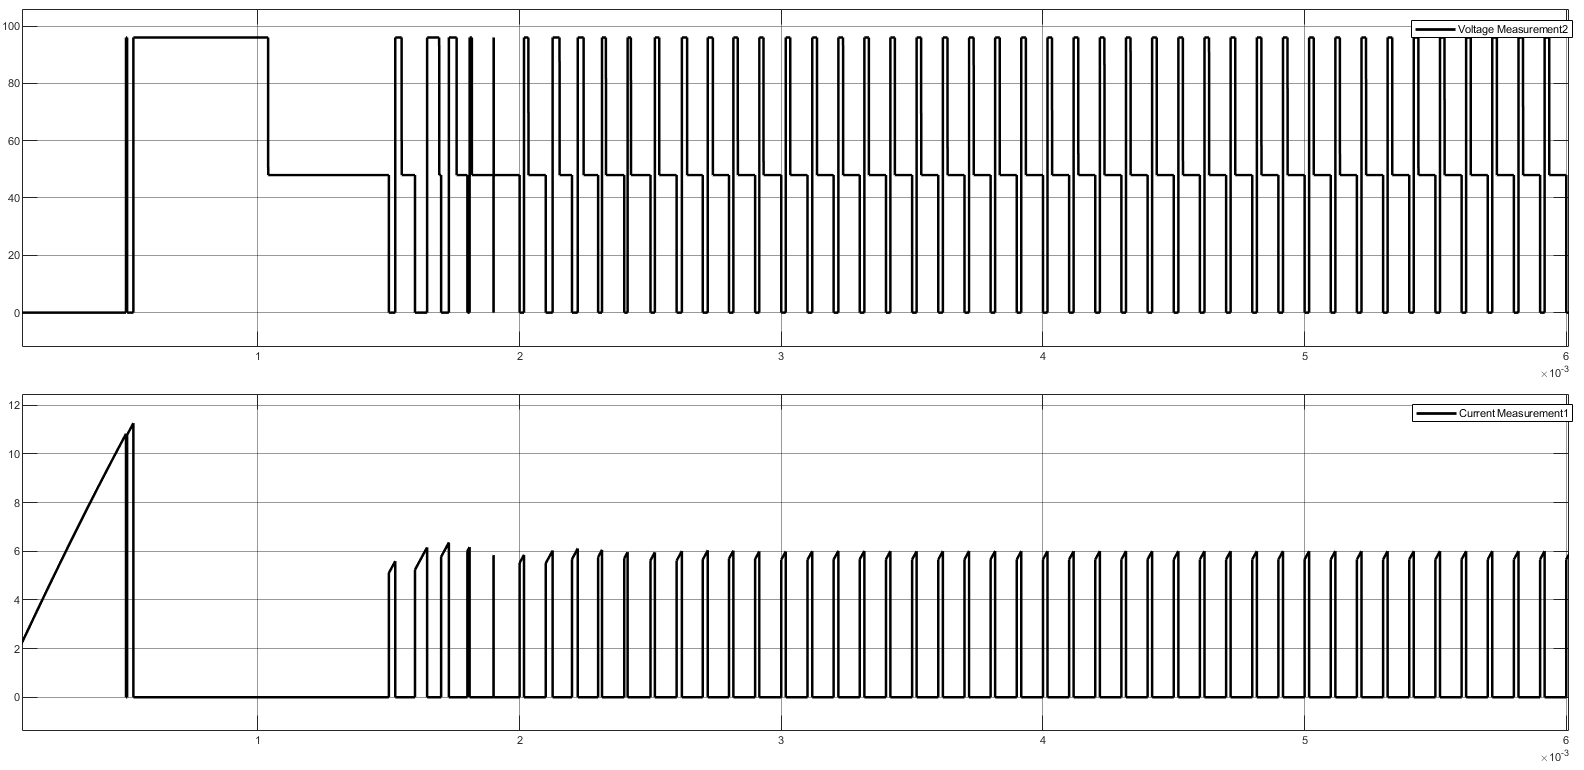
\includegraphics[scale=0.35]{mosfet.png}
    \caption{Voltage and current wave forms of mosfet when input 48V}
    \label{fig:my_label}
\end{figure}
\tap Duty cycle signal statistics are shown below. 
\begin{figure}[H]
    \centering
    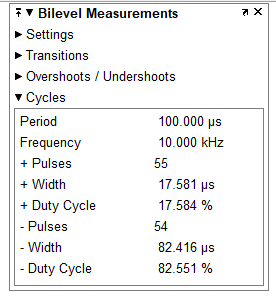
\includegraphics[scale=0.8]{duty48.PNG}
    \caption{Duty cycle signal information when input is equal to 48V}
    \label{fig:my_label}
\end{figure}
\tab We measure also diodes voltages and currents because diodes ratings are also important.Diodes currents and voltages shown below.

\begin{figure}[H]
    \centering
    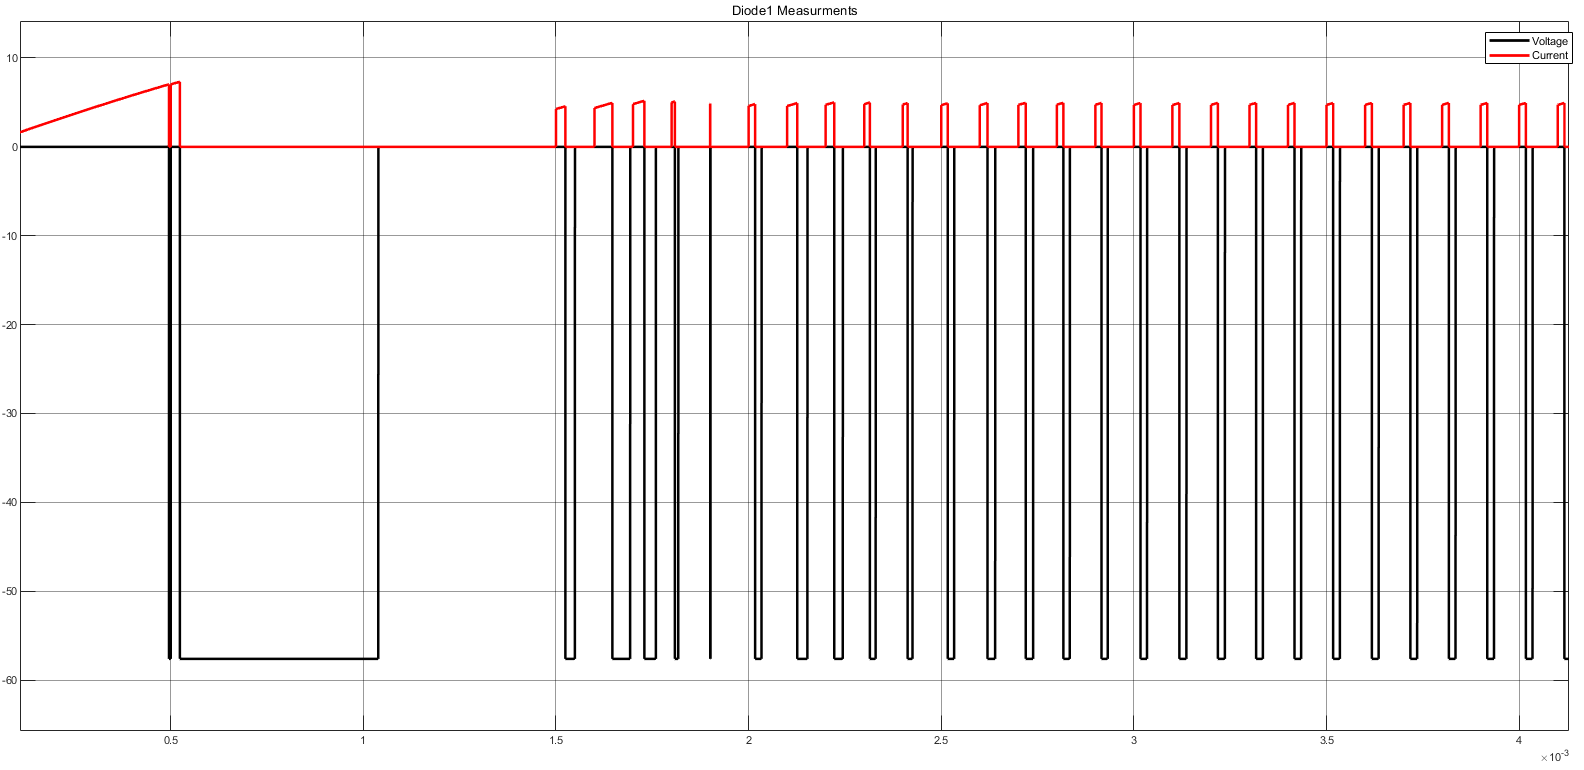
\includegraphics[scale=0.3]{diode1.png}
    \caption{Voltage and current wave forms of diode 1 when input 48V}
    \label{fig:my_label}
\end{figure}

\begin{figure}[H]
    \centering
    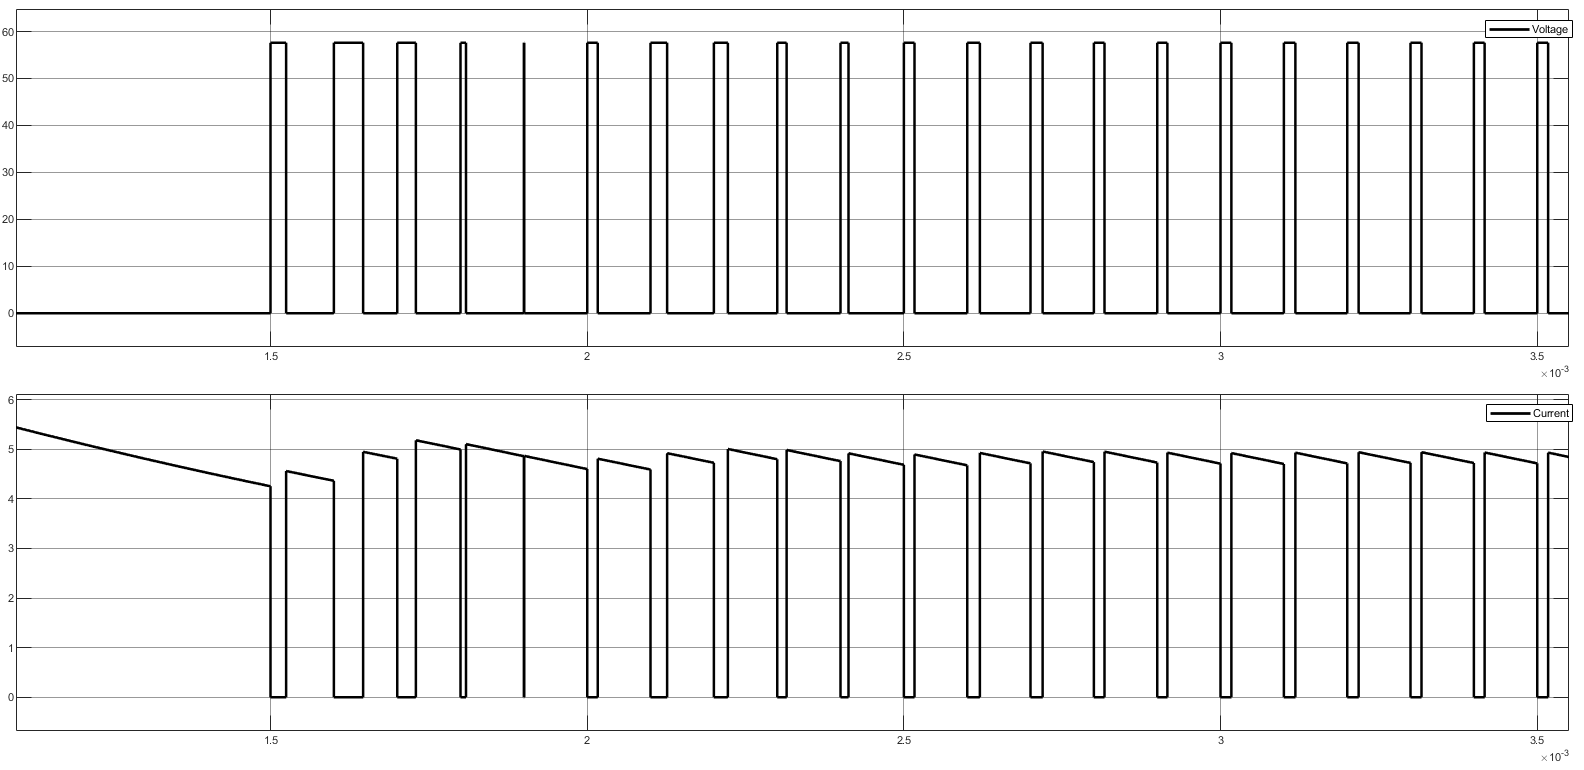
\includegraphics[scale=0.3]{48diode2.png}
    \caption{Voltage and current wave forms of diode 2 when input 48V}
    \label{fig:my_label}
\end{figure}

\begin{figure}[H]
    \centering
    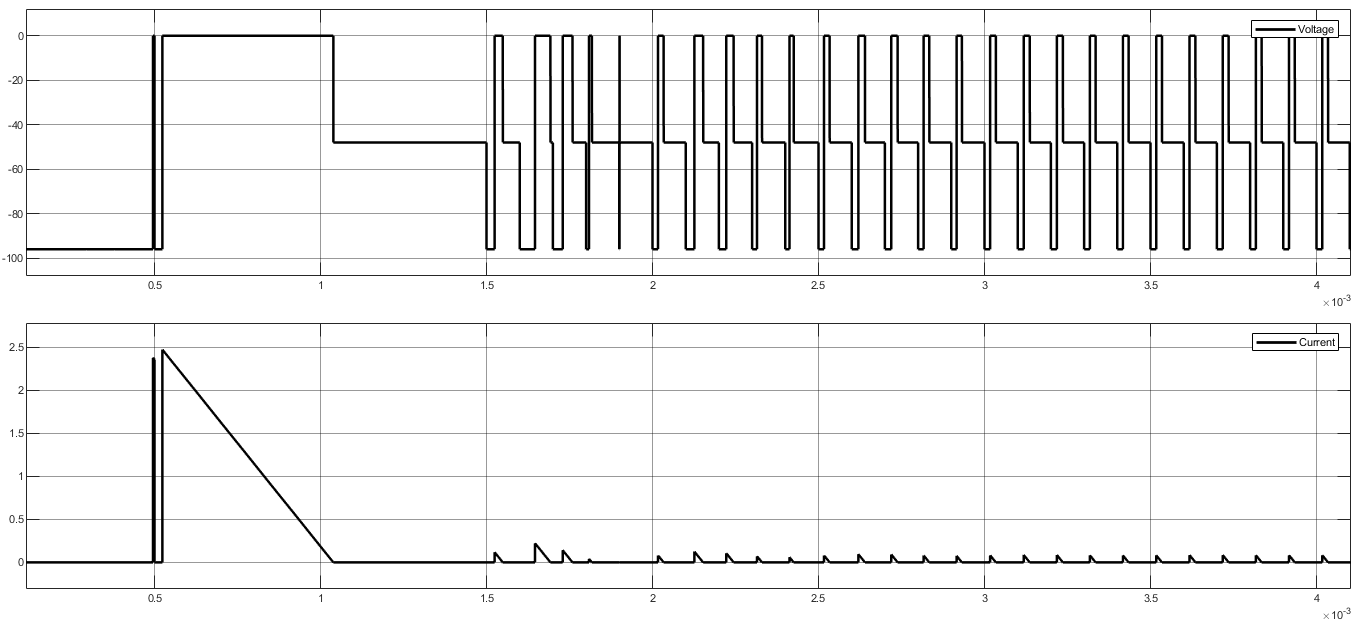
\includegraphics[scale=0.3]{48diode3.png}
    \caption{Voltage and current wave forms of diode 3 when input 48V}
    \label{fig:my_label}
\end{figure}
\tab We also measure the output capacitor voltages and current for component selection
\begin{figure}[H]
    \centering
    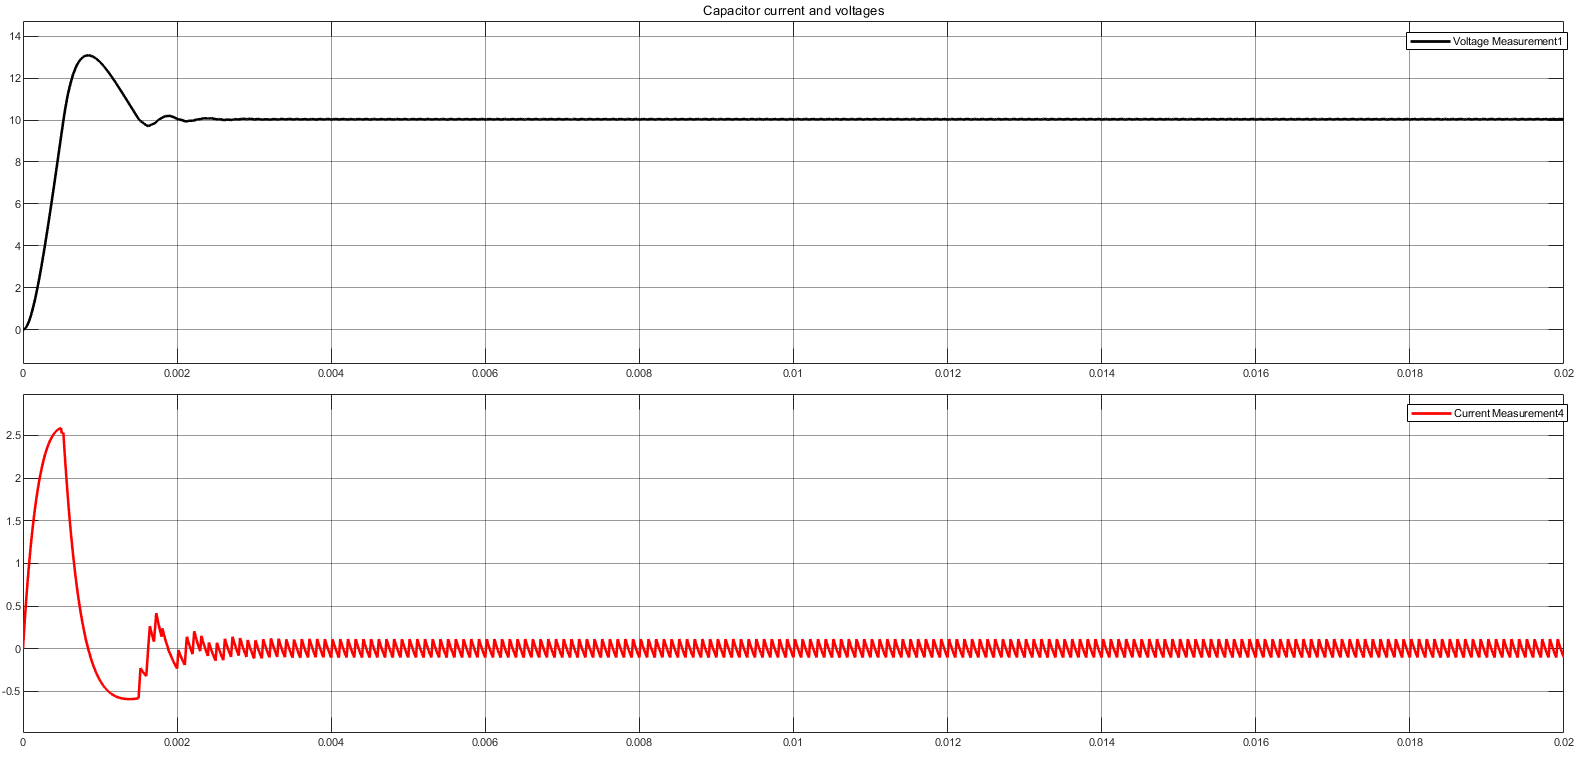
\includegraphics[scale=0.3]{capacitor48.png}
    \caption{Voltage and current wave forms of capacitor when input 48V}
    \label{fig:my_label}
\end{figure}
\textbf{b)} We simulated circuit when input is equal to 24V.  We simulate extreme point of the specifications. Output wave form of the converter shown below.

\begin{figure}[H]
    \centering
    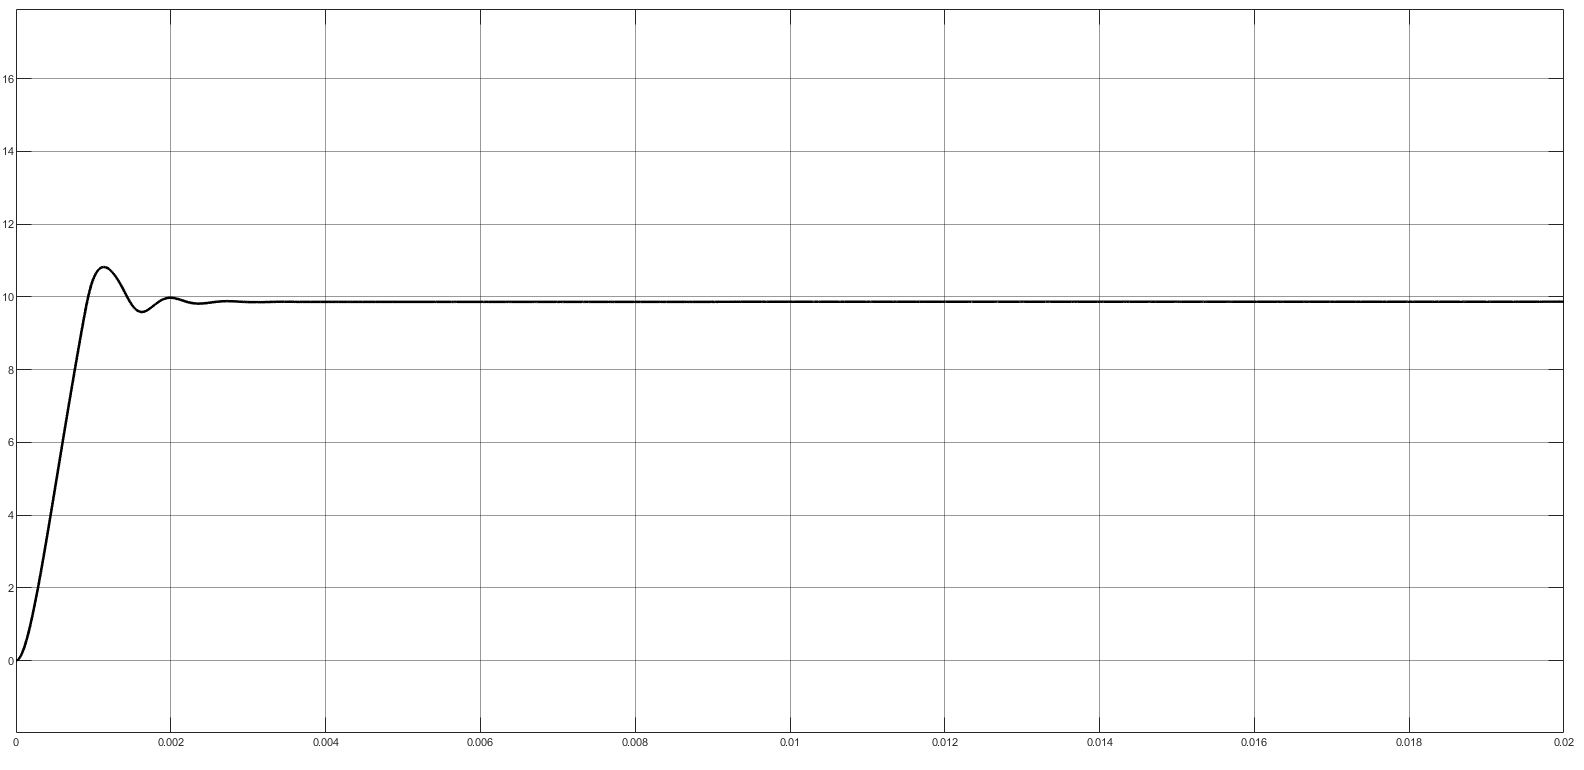
\includegraphics[scale=0.3]{24in.png}
    \caption{Output waveform when input is 24V}
    \label{fig:my_label}
\end{figure}
\tab When input is equal to 24V, our duty cycle must be at the highest value due to the specifications.Our highest duty cycle is $\%$34.250. $\%$34.250 duty cycle give us 10V when input is 24V.Signal statistics of the output waveform is shown below.
\begin{figure}[H]
    \centering
    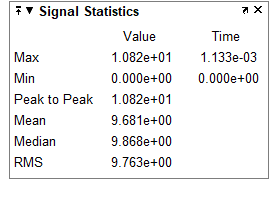
\includegraphics[scale=0.9]{24sinyal.PNG}
    \caption{Output waveform signal statistics when input is 24V}
    \label{fig:my_label}
\end{figure}
\begin{figure}[H]
    \centering
    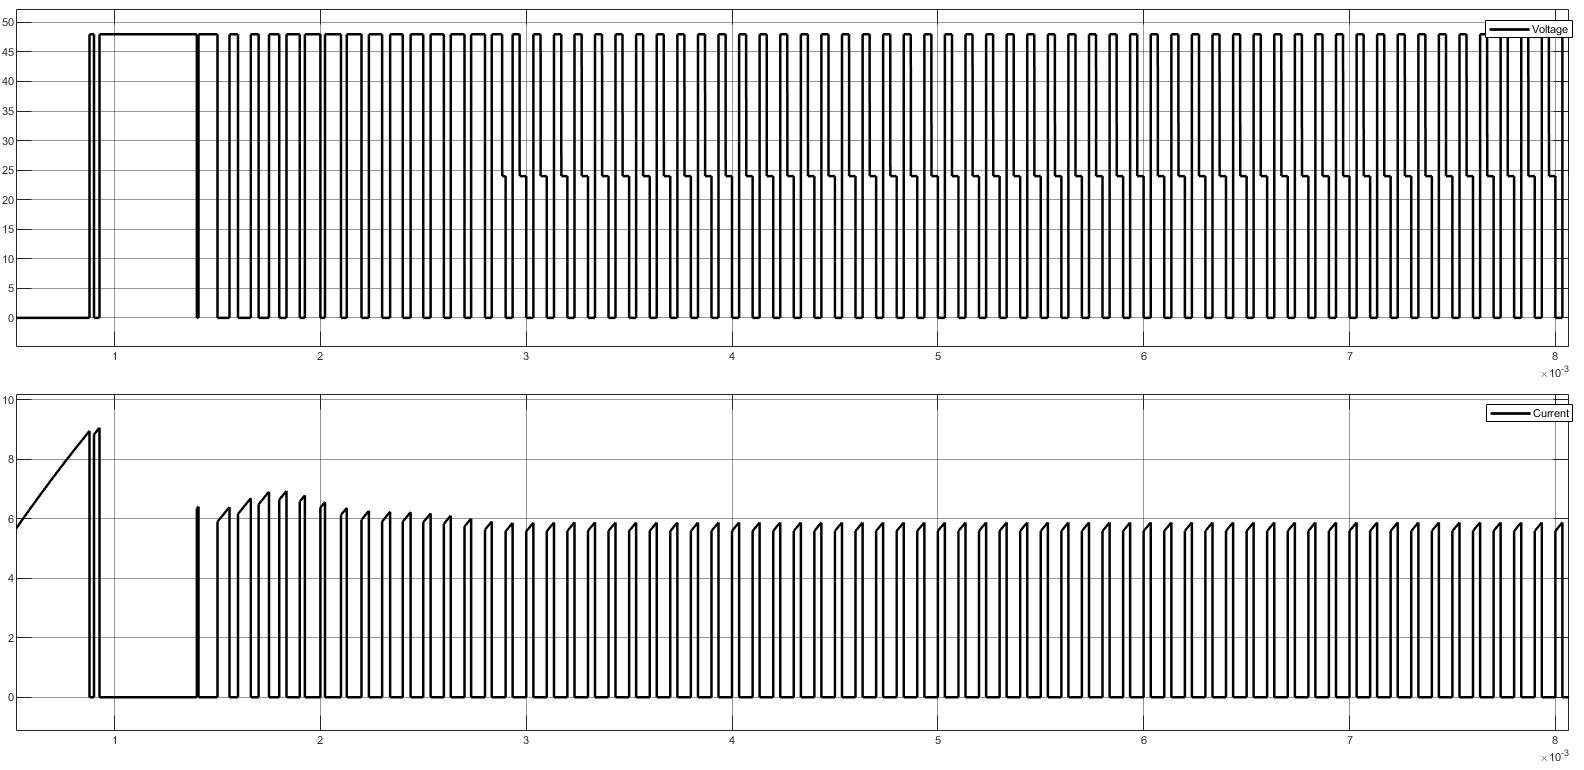
\includegraphics[scale=0.3]{mosfet2.png}
    \caption{Voltage and current waveforms of mosfet when input 24V}
    \label{fig:my_label}
\end{figure}
\tab According to simulation results, mosfet should be capable of handling $96 V$ drain to source voltage and $6 A$ current. As a result, we chose  \href{https://pdf.direnc.net/upload/irf540nspbf-datasheet.pdf}{IRF540 N} as our transistor with $100 V$ and $27 A$ ratings.

\tap When input is equal to 24V duty cycle signal information shown below.

\begin{figure}[H]
    \centering
    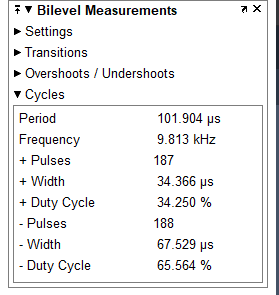
\includegraphics[scale=0.9]{duty24.PNG}
    \caption{Duty cycle signal information when input is equal to 24V}
    \label{fig:my_label}
\end{figure}
\tab When input equal to 24V diodes voltages and currents are shown below. 
\begin{figure}[H]
    \centering
    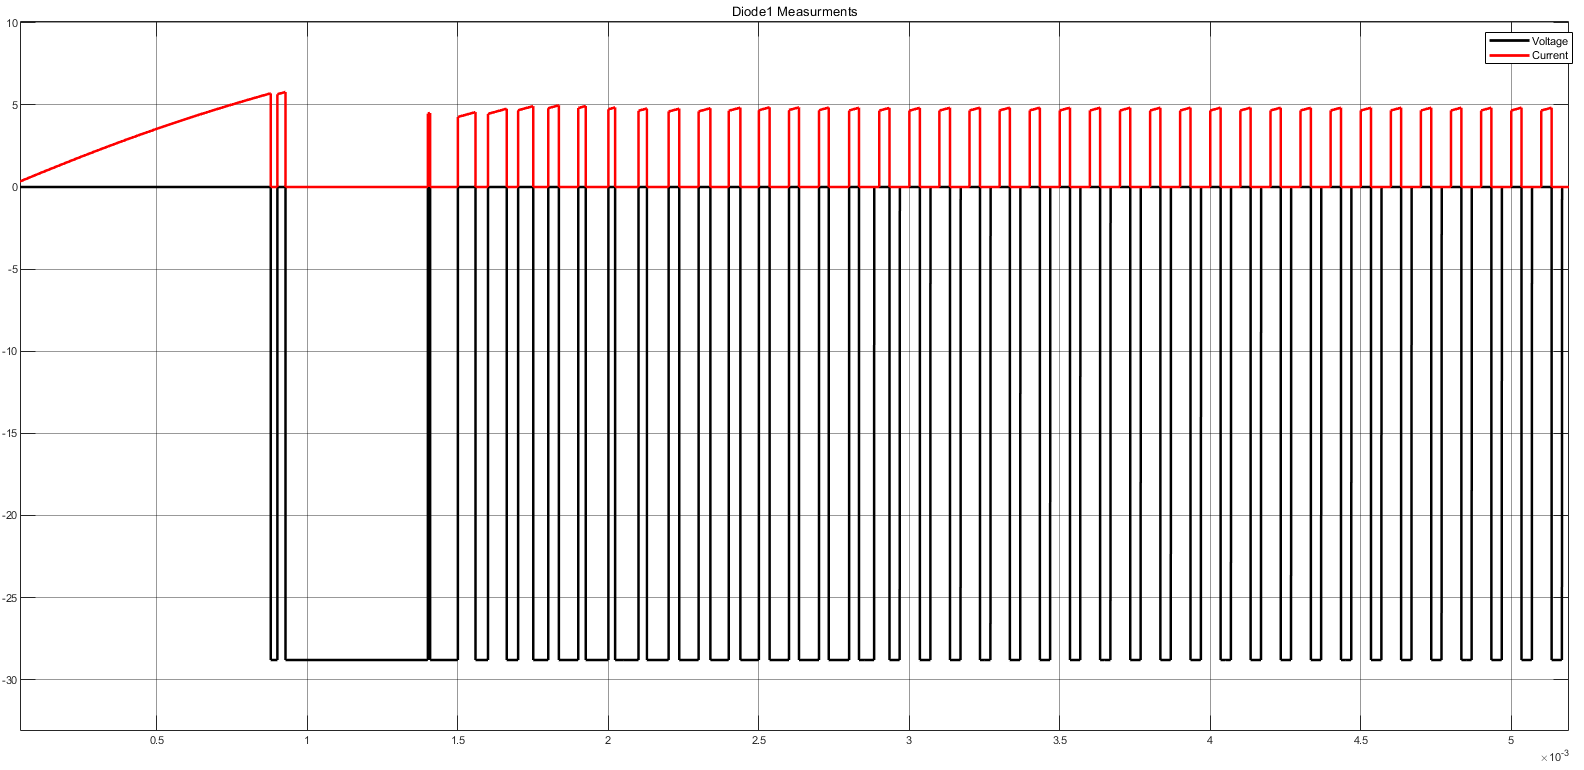
\includegraphics[scale=0.3]{24diode1.png}
    \caption{Voltage and current waveforms of diode 1 when input 24V}
    \label{fig:my_label}
\end{figure}

\begin{figure}[H]
    \centering
    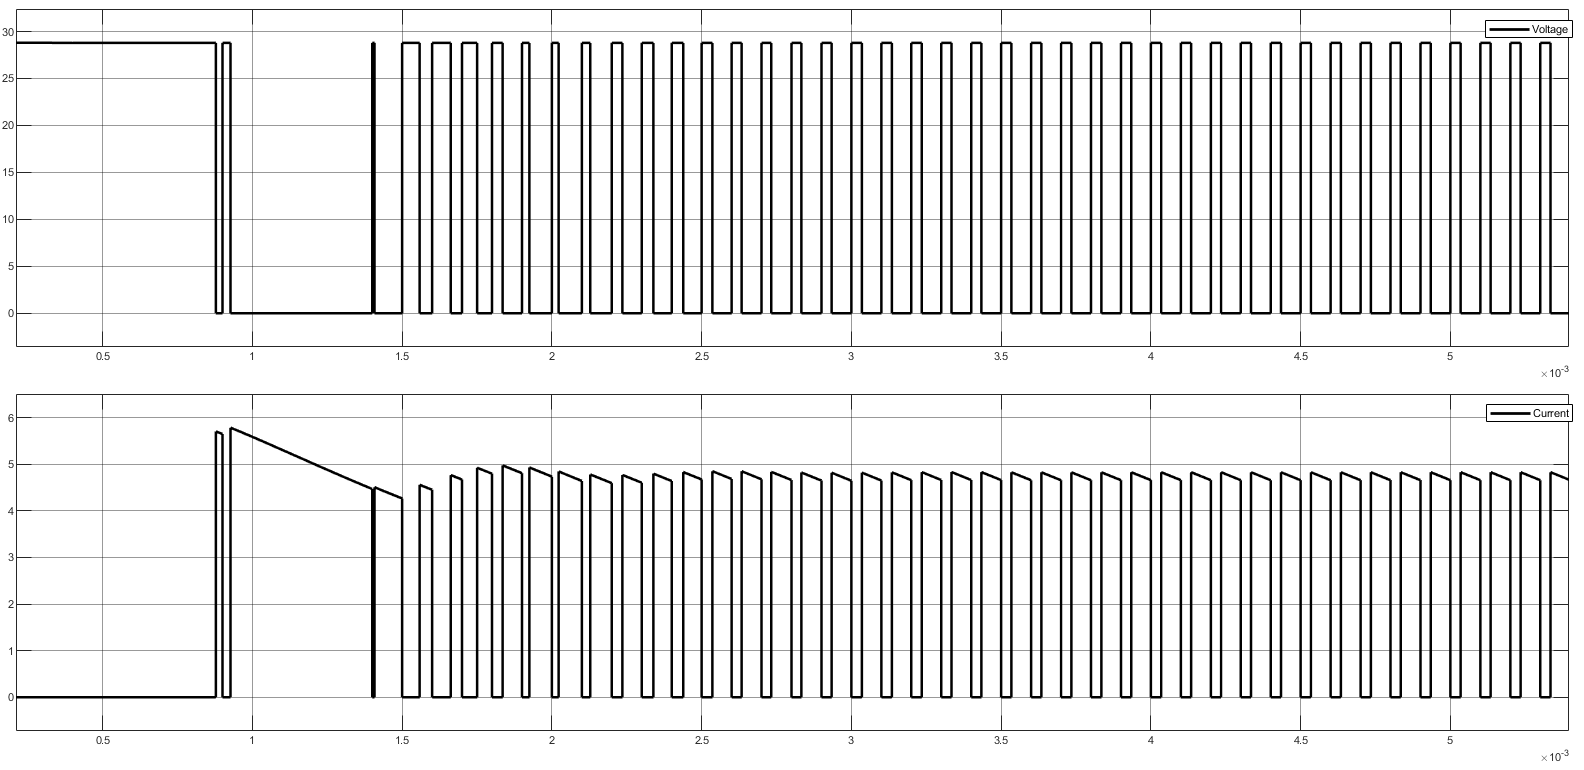
\includegraphics[scale=0.3]{24diode2.png}
    \caption{Voltage and current waveforms of diode 2 when input 24V}
    \label{fig:my_label}
\end{figure}

\begin{figure}[H]
    \centering
    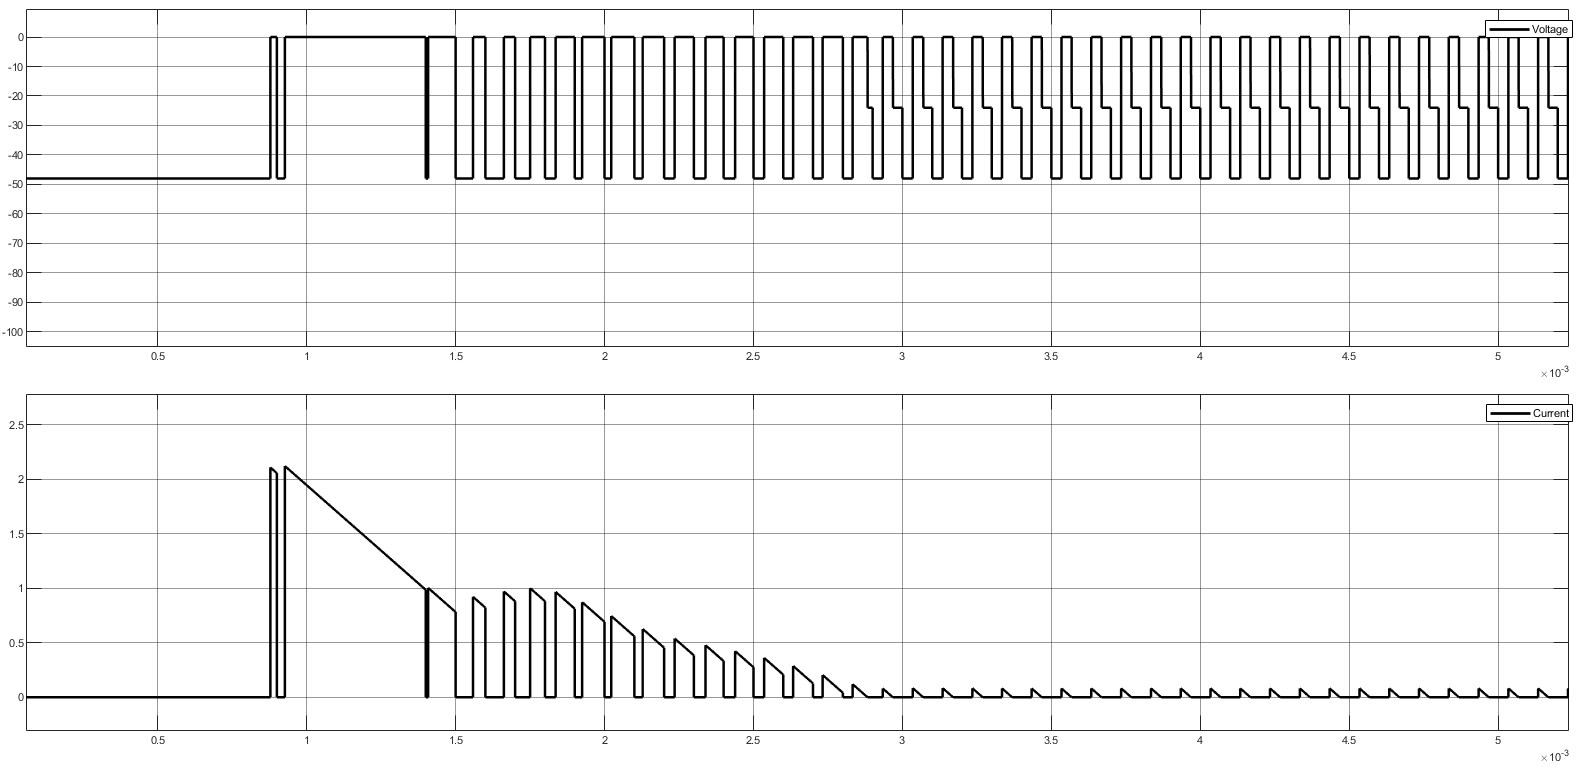
\includegraphics[scale=0.3]{24diode3.png}
    \caption{Voltage and current wave forms of diode 3 when input 24V}
    \label{fig:my_label}
\end{figure}

\tab Diodes on the output side have same voltage and current stresses, which are $58 V$ and $6 A$. Diode on the input side has $96 V$ and $2.5 A$ ratings. We decided to use same \href{https://www.direnc.net/mbr20100-diyot--20a-100v-dual-high-voltage-schottky}{MBR20100} diode for all of them whose ratings are $100 V$ and $20 A$. Since this diode is Schottky it is beneficial to use it since there is no recovery time in Schottky diodes.

\begin{figure}[H]
    \centering
    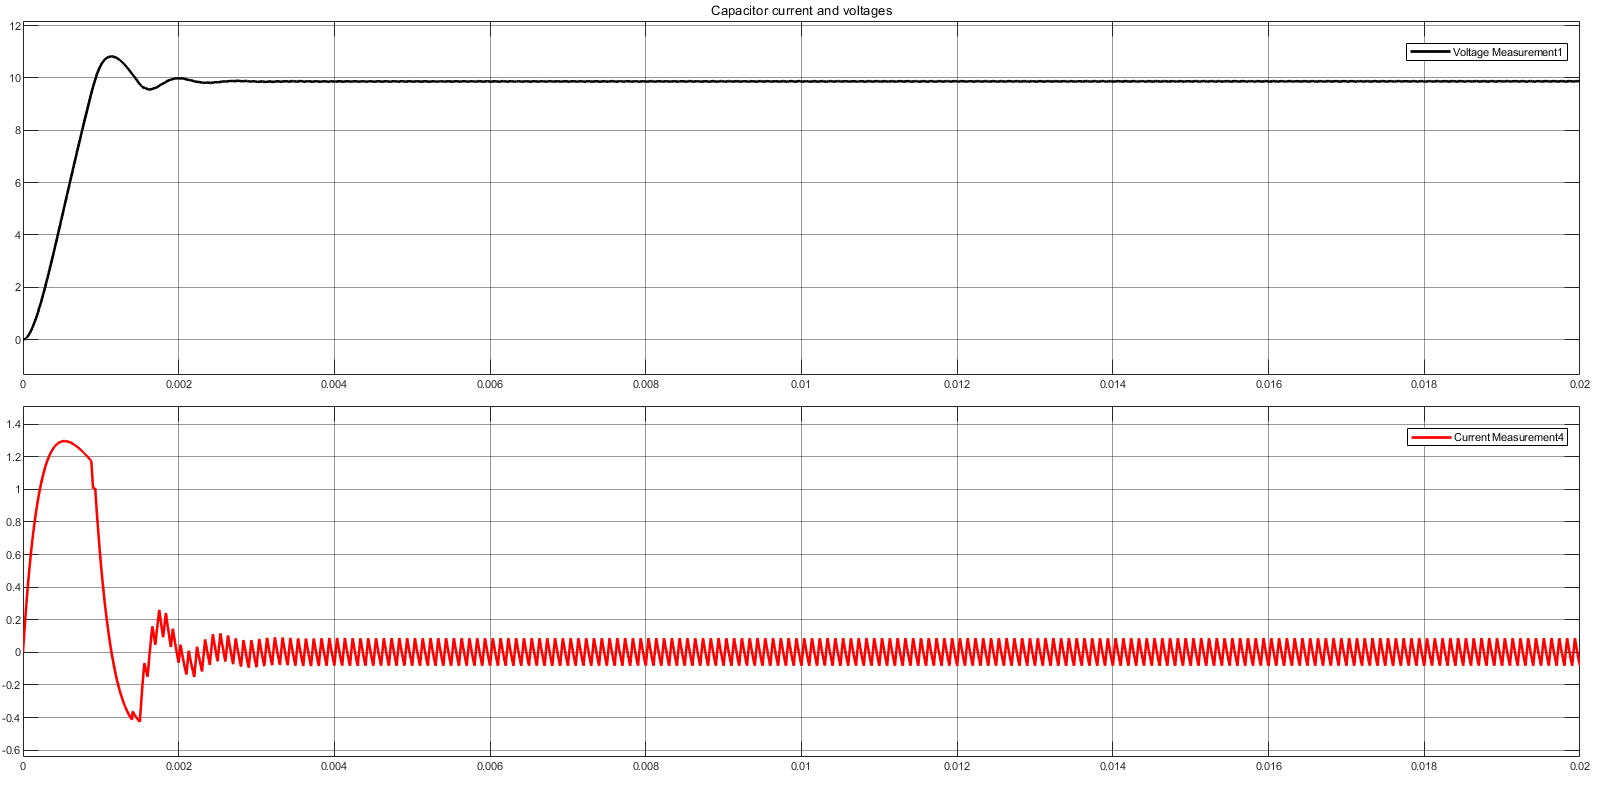
\includegraphics[scale=0.3]{capacitor24.png}
    \caption{Voltage and current wave forms of capacitor when input 24V}
    \label{fig:my_label}
\end{figure}
\tab In capacitor selection, we desired to have a capacitor with a high capacitance rating so that it can reduce output voltage ripple to desired levels and we also wanted it to withstand the output voltage with a safe difference between capacitor rating and output voltage. Another thing we considered is minimizing the ESR value since we do not want to reduce our efficiency. As a result, \href{https://www.digikey.com/product-detail/en/kemet/ESC107M016AC3AA/399-6080-ND/2712569}{ESC107M016AC3AA} is selected. It has $100 µF$ capacitance and $16 V$ voltage rating. Its ESR value is specified as $900 mOhm$ at $100 KHz$. We expect it to be lower at our case since our switching frequency is $10 KHz$.

\newpage
\section*{Conclusion}
\tab In this report, we specified our decisions and plans to build a Forward Converter which can meet the criteria that are specified in project definition.Firstly, we made some calculations considering our design specifications and then we simulated our design and observed stresses on the components, non-ideal behaviors of them and how they affect our requirements.
\newline\tab To conclude, we believe this report is going to be helpful once we start to implement our design since we considered not only ideal case like in the simulation, but also many non-ideal situations such as fill factor, saturation of the core etc. We became more prepared for the actual project with the help of this report.


\end{document}